\documentclass[12pt,a4paper]{article}

\usepackage[T1]{fontenc} 
\usepackage[utf8]{inputenc}

\usepackage[a4paper]{geometry}
\geometry{hscale=0.85,vscale=0.85,centering}
\usepackage{lmodern}
\usepackage{framed}
\usepackage[framed]{ntheorem}
\usepackage{xcolor}
\usepackage{graphicx}
\usepackage{tikz}
\usepackage{subfigure}
\usepackage{wrapfig}
\graphicspath{ {./img/} }
\usepackage{amssymb}
\usepackage{amsmath}
\usepackage{amsfonts}
\usepackage{dsfont}
\usepackage{listings}
\usepackage{titlesec}
\usepackage{pgfplots}
\pgfplotsset{compat=1.12}
\usepackage{url}
\usepackage{hyperref}
\hypersetup{					% setup the hyperref-package options
	breaklinks=true,			% 	- allow line break inside links		%
	colorlinks,
	citecolor=black,
	filecolor=black,
	linkcolor=black,
	urlcolor=black
}

\usepackage[francais]{babel}


\titleformat{\section}
{\centering \Large \normalfont \scshape}{\thesection}{1em}{}
\titleformat{\subsection}
{ \large \scshape}{\thesubsection}{1em}{}
\titleformat{\subsubsection}
{ \normalsize \scshape}{\thesubsubsection}{1em}{}
\numberwithin{equation}{section}

\setcounter{tocdepth}{2}

\newcommand{\elevation}{\texttt{Elevation}}
\newcommand{\aspect}{\texttt{Aspect}}
\newcommand{\slope}{\texttt{Slope}}
\newcommand{\hhydro}{\texttt{Horizontal\_Distance\_To\_Hydrology}}
\newcommand{\vhydro}{\texttt{Vertical\_Distance\_To\_Hydrology}}
\newcommand{\roadways}{\texttt{Horizontal\_Distance\_To\_Roadways}}
\newcommand{\hilshadeM}{\texttt{Hilshade\_9am}}
\newcommand{\hilshadeN}{\texttt{Hilshade\_Noon}}
\newcommand{\hilshadeA}{\texttt{Hilshade\_3pm}}
\newcommand{\fire}{\texttt{Horizontal\_Distance\_To\_Fire_Points}}
\newcommand{\wilderness}{\texttt{Wilderness\_Area}}
\newcommand{\soil}{\texttt{Soil\_Type}}
\newcommand{\cover}{\texttt{Cover\_Type}}

\title{\scshape \huge Forest Cover Type Prediction}
\author{\textbf{Kevin Zagalo} \\  \url{kevin.zagalo@etu.upmc.fr}  \and \textbf{Ismail Benkirane} \\ \url{ismail.benkirane@etu.upmc.fr}}
\date{}

\begin{document}

	\maketitle
	
{\small Projet pour le cours \textit{Apprentissage Statistique} du LIP6 \footnote[0]{Laboratoire d'Informatique de Paris 6 :: \url{https://www.lip6.fr}}, Sorbonne Université} \hfill Janvier 2019
	
	\hrulefill

	\begin{abstract}
		  Ce projet a pour but de proposer et tester des modèles pour l'étude de la base de données  \textit{Covertype} \footnote{\url{https://archive.ics.uci.edu/ml/datasets/Covertype}}. Il s'agit d'un problème de classification multi-classe avec 7 classes, et 581\,012 instances de 54 attributs sans données manquantes. 
	\end{abstract}

	\hrulefill

	\tableofcontents
	
	\newpage
	
	\section{Chargement des données}
	
	On choisit d'utiliser la bibliothèque \verb!pandas! pour charger les données, surtout pour l'analyse préliminaire. \verb!pandas! fournit une panoplie de fonctions pour visualiser les données. \verb!groupby!, \verb!boxplot! et \verb!hist! nous seront forts utiles pour choisir les données que nous exploiterons. Le \textit{notebook} contenant le code joint au rapport nécessite aussi les bibliothèques \verb!matplotlib!, \verb!numpy!, \verb!sklearn! et \verb!plotly!.\\
	
	Les attributs sont les suivants : 
	
	\begin{flushleft}
		\begin{tabular}{l l p{5.2cm}}
			Nom & Unité & Description \\
			\hline
			\elevation & mètres & Altitude \\ 
			\aspect & degrés & Orientation \\ 
			\slope & degrés & Pente \\
			\hhydro & mètres & Distance horizontale au point d’eau le plus proche\\
			\vhydro & mètres & Distance verticale au point d’eau le plus proche \\
			\roadways & mètres & Distance horizontale à la route la plus proche \\
			\hilshadeM & entier entre 0 et 255 & Ombrage à 9h au solstice d’été \\
			\hilshadeN & entier entre 0 et 255 & Ombrage à 12h au solstice d'été\\
			\hilshadeA & entier entre 0 et 255 &  Ombrage à 15h au solstice d'été \\
			\verb!Horizontal_Distance_To_Fire_Points! & mètres & Distance horizontale au départ de feu le plus proche\\
			\wilderness & 4 colonnes binaires & Wilderness area designation \\
			\soil & 40 colonnes binaires & Type de sol\\
			\cover & entier entre 1 et 7 & Classe\\
		\end{tabular}
	\end{flushleft}

	Le problème de ce chargement est qu'il stocke les données en type \verb!str!, il nous faut donc convertir le type des données. C'est ce que font les fonctions \verb!convert_to_listofbool!, \verb!convert_to_int! et \verb!convert_to_float!. \\
	
	On préfèrera garder dans le DataFrame \verb!df_covtype! des entiers plutôt que des vecteurs binaires, quitte à les y remettre dans les données de train et de test ensuite. Cela facilitera grandement l'analyse préliminaire. On utilisera donc \verb!wilderness! et \verb!soil! uniquement pour la partie test des modèles.\\
	
	Nos données seront donc : 
	\begin{itemize}
	 	\item \verb!df_covtype! : \textit{DataFrame} de toutes les données non traitées triées par attributs. 
	 	\item \verb!df_bycovtype! : \textit{DataFrame.groupby} de toutes les données triées par attributs et regroupée par classes. 
	 	\item \verb!labels! :\textit{np.array} des étiquettes des types de forêts.
	 	\item \verb!dict_attributs! : \textit{dictionnaire} qui associe les attributs aux bons index. 
	 	\item \verb!qualitative! : \textit{liste} des attributs des données qualitatives.
	 	
	 	\begin{itemize}
	 		\item \wilderness :
	 	
		 		\begin{itemize}
		 				\item 1 : Rawah Wilderness Area
		 				\item 2 : Neota Wilderness Area
		 				\item 3 : Comanche Peak Wilderness Area
		 				\item 4 : Cache la Poudre Wilderness Area
		 		\end{itemize}
		 	
		 	\item \soil :
		 	\begin{itemize}
		 		\item 1 to 40 : based on the USFS Ecological Landtype Units for this study area
		 	\end{itemize}
	 	
	 		\item \verb!forest_cover_types! : 
	 			\begin{itemize}
	 					\item 1 : Spruce/Firze
 						\item 2 : Lodgepole Pine
 						\item 3 : Ponderosa Pine
 						\item 4 : Cottonwood/Willow
 						\item 5 : Aspen
 						\item 6 : Douglas-fir
 						\item 7 : Krummholz
		\end{itemize}
	\end{itemize}
	
	\item \verb!wilderness! et \verb!soil! : \textit{listes} gardant en mémoire les vecteurs binaires pour les remplacer par des entiers. On garde donc les 44 paramètres de ces attributs dans notre modèle.
	
	\end{itemize}
	
	\section{Analyse préliminaire et pré-traitement des données}
	
	Tout d'abord on constate sur la figure \ref{fig:datahist} que les données sont inégalement réparties selon les classes. Cela peut vouloir dire plusieurs choses : soit nos données sont mal échantillonnées, soit les types \verb!1! et \verb!2! sont effectivement largement plus répandues.\\
	
	\begin{wrapfigure}{r}{0.65\textwidth}
		\centering
		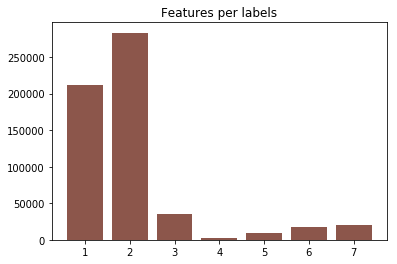
\includegraphics[width=1\linewidth]{img/data_hist}
		\caption{Histogramme des données par types de forêts}
		\label{fig:datahist}
	\end{wrapfigure}

	 C'est quelque chose dont nous n'avons pas la maitrise, une discussion avec un expert sur le sujet serait préférable. Nous continuerons l'étude sans experts et en supposant que les données sont raisonnablement échantillonnées.\\
	
	La suite consistera globalement à faire la même chose sur le reste des données grâce aux méthodes de la bibliothèque \verb!pandas!.\\
	
	\begin{figure}[h]
		\centering
		\subfigure[Slope]{
			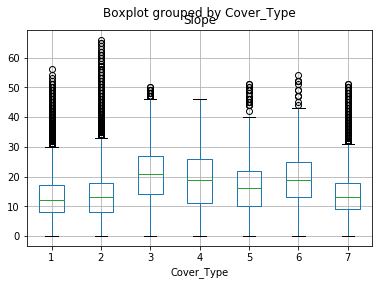
\includegraphics[width=0.3\linewidth]{img/slope_boxplot}
		}
		\hfill
		\subfigure[Aspect]{
			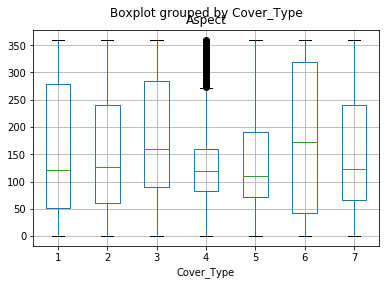
\includegraphics[width=0.3\linewidth]{img/aspect_boxplot}
		}
		\hfill
		\subfigure[Elevation]{
			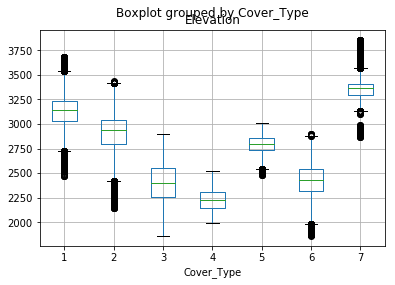
\includegraphics[width=0.3\linewidth]{img/elevation_boxplot}
		}
		\hfill
		\subfigure[Horizontal distance to hydrology]{
			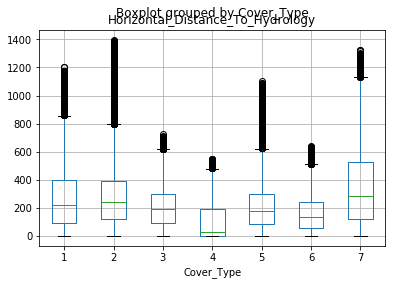
\includegraphics[width=0.22\linewidth]{img/Horizontal_Hydrology_boxplot}
		}
	\hfill
		\subfigure[Distance to roadways]{
			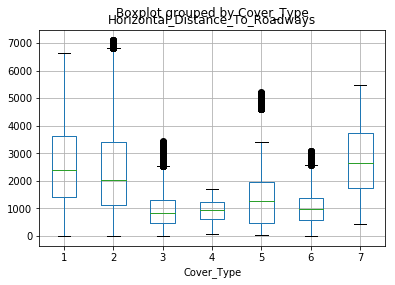
\includegraphics[width=0.22\linewidth]{img/roadways_boxplot}
		}
	\hfill
		\subfigure[Distance to fire points]{
			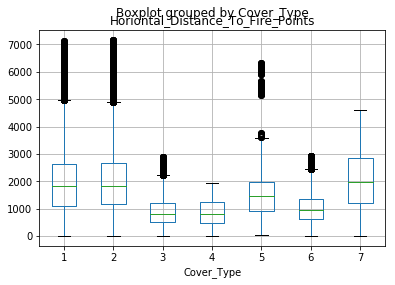
\includegraphics[width=0.22\linewidth]{img/fire_boxplot}
		}
	\hfill
		\subfigure[Hillshade at 3pm]{
			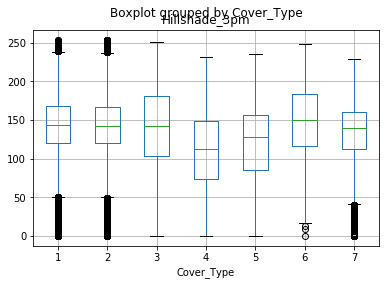
\includegraphics[width=0.22\linewidth]{img/Hillshade_3pm_boxplot}
		}
		\caption{Boxplot des données numériques}
		\label{fig:boxplots}
	\end{figure}
	
	On observe dans la figure \ref{fig:boxplots} l'importance des attributs \elevation, \slope et \aspect. On voit aussi la très faible variation de \vhydro. Pour ce qui est des attributs concernant l'ombrage au solstice, on pourra chercher un lien de corrélation pour réduire à une seule variable le triplet de données \hilshadeM, \hilshadeN, \hilshadeA.\\
	
	La première partie consistera donc à voir si on peut réduire le nombre de paramètres, la deuxième à modifier les données pour une meilleure analyse, et enfin mettre les données de train, de validation et de test. On trouve déjà quelques idées dans \cite{B-D}.
	
	\newpage
	
	\subsection{Réduction des paramètres}
	
	Tout d'abord, nous nous contenterons de la distance au point d'eau le plus proche, c'est à dire du nouvel attribut \verb!Distance_To_Hydrology! définie par la distance euclidienne entre la forêt et le point d'eau, c'est-à-dire la quantité $$ \sqrt{ \vhydro^2 +  \hhydro^2}$$
	
	\begin{figure}[h]
		\centering
		\subfigure[Vertical distance to hydrology]{
			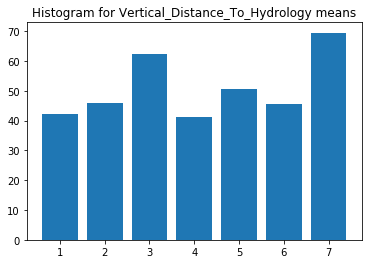
\includegraphics[width=0.3\linewidth]{img/vhydrohist}
		}
		\hfill
		\subfigure[Horizontal distance to hydrology]{
			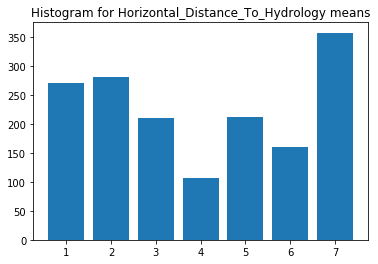
\includegraphics[width=0.3\linewidth]{img/hhydrohist}
		}
		\hfill
		\subfigure[Distance to hydrology]{
			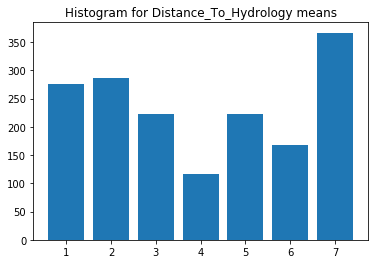
\includegraphics[width=0.3\linewidth]{img/hydrohist}
		}
	\caption{Histogrammes des distances moyennes au point d'eau le plus proches par types de forêts}
	\label{fig:disthist}
	\end{figure}
	
	En effet, lorsqu'on regarde la figure \ref{fig:disthist}, on constate que ce nouvel attribut reste similaire à \hhydro tout en étant sensible aux variations de\\ \vhydro.\\

	
	Ensuite, 
	
	\newpage

	
	\subsection{Données qualitatives}
	Premièrement, au vu du nombre de paramètres que comportent les attributs \soil et \wilderness, on peut se demander si ces données sont vraiment utiles au problème,
	
	
	
	\begin{figure}[h]
		\centering
		\subfigure[Classe 1]{
			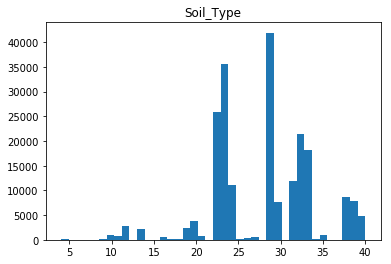
\includegraphics[width=0.3\linewidth]{img/soil1}
		}
	\hfill
		\subfigure[Classe 2]{
			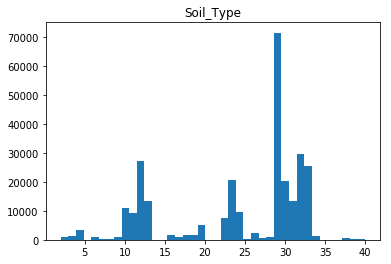
\includegraphics[width=0.3\linewidth]{img/soil2}
		}
	\hfill
		\subfigure[Classe 3]{
			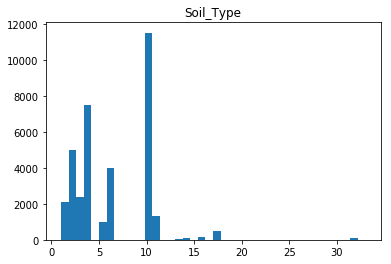
\includegraphics[width=0.3\linewidth]{img/soil3}
		}

	\medskip
	
	\subfigure[Classe 4]{
		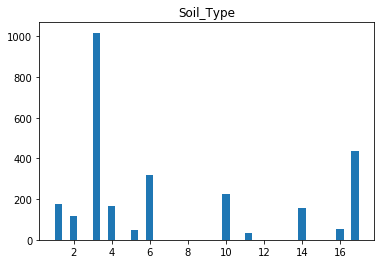
\includegraphics[width=0.22\linewidth]{img/soil4}
	}
	\subfigure[Classe 5]{
		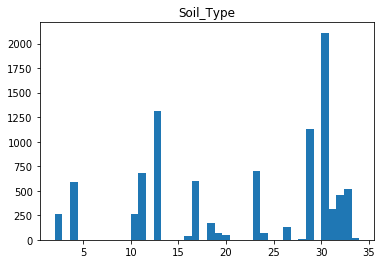
\includegraphics[width=0.22\linewidth]{img/soil5}
	}
	\subfigure[Classe 6]{
		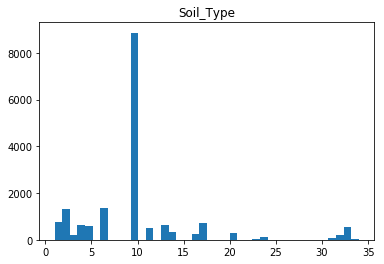
\includegraphics[width=0.22\linewidth]{img/soil6}
	}
	\subfigure[Classe 7]{
		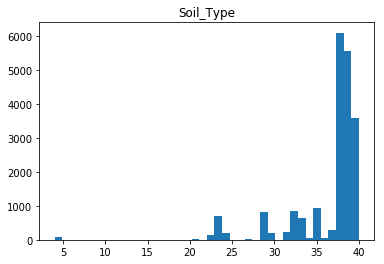
\includegraphics[width=0.22\linewidth]{img/soil7}
	}

		\subfigure[Classe 1]{
			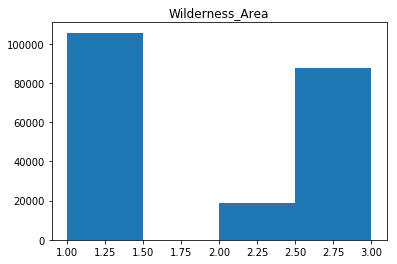
\includegraphics[width=0.3\linewidth]{img/wilderness1}
		}
		\hfill
		\subfigure[Classe 2]{
			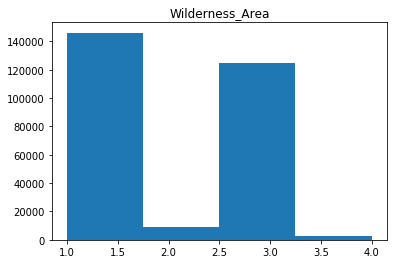
\includegraphics[width=0.3\linewidth]{img/wilderness2}
		}
		\hfill
		\subfigure[Classe 3]{
			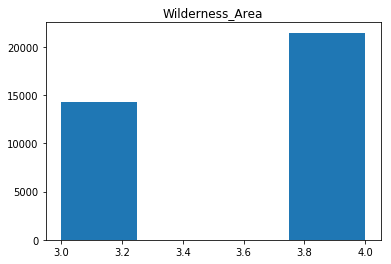
\includegraphics[width=0.3\linewidth]{img/wilderness3}
		}
		
		\medskip
		
		\subfigure[Classe 4]{
			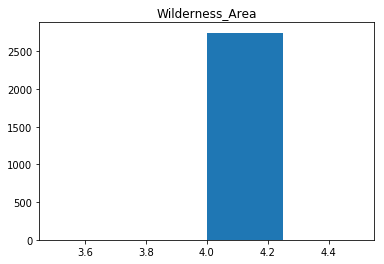
\includegraphics[width=0.22\linewidth]{img/wilderness4}
		}
		\subfigure[Classe 5]{
			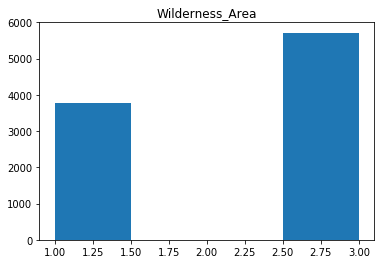
\includegraphics[width=0.22\linewidth]{img/wilderness5}
		}
		\subfigure[Classe 6]{
			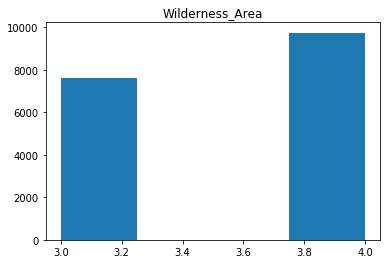
\includegraphics[width=0.22\linewidth]{img/wilderness6}
		}
		\subfigure[Classe 7]{
			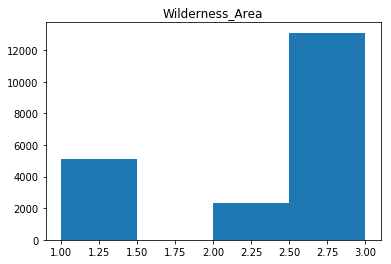
\includegraphics[width=0.22\linewidth]{img/wilderness7}
		}
		\caption{Distributions de \soil (a)--(g) et \wilderness (h)--(n) par classes de forêts}
		\label{fig:soil-wild_hist}
	\end{figure}
	
	et effectivement les données qualitatives sont importantes : on voit sur la figure \ref{fig:soil-wild_hist} qu'elles varient beaucoup selon les classes, et dans \cite{C-D} qu'elles changent considérablement le score des modèles \textit{K-Means} et \textit{SVM}.
	
	\newpage
	
	\section{Test des méthodes}
	
	\subsection{k-plus proches voisins}
	
	L'apprentissage prend un temps fou...
	
	\subsection{Random Forest}
	
	On fait varier les paramètres de notre premier modèle. On commence par le paramètre \texttt{n\_variables}, \\
	
	
	
	\begin{figure}[h]
		\centering
		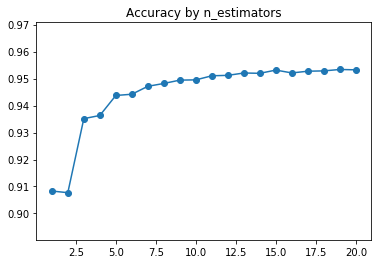
\includegraphics[width=0.7\linewidth]{img/random_forest_accuracy1}
		\caption{Accuracy en fonction du paramètre \texttt{n\_variables} }
		\label{fig:randomforestaccuracy1}
	\end{figure}
	
	
	
	\bibliographystyle{alphadin}
	\bibliography{covtype}
	
	\end{document}